\chapter{Critiques of the Soundscape Circumplex}
\label{app:CircCritique}

\subsection{Application \& Simulations}
In order to investigate the shape of the circumplex coordinate space generated by this transformation, a dataset of 3 million randomly simulated PA responses was generated. For each of the 8 PAs, an integer value from 1 to 5 is randomly generated from a uniform distribution, meaning each of the five responses is equally likely. These simulated data are specifically not intended to include any information about correlations between the various PAs when actually answered by respondents (see \citep{Lionello2021Introducing} for more on this discussion), instead the PA responses are completely uncorrelated as they each have their own random distribution. Therefore, the simulated dataset represents a theoretical uniform coverage of the 8 dimensional PA space.

We then apply the ISO transformations given in \cref{eqn:pleasant,eqn:eventful}, resulting in 3 million coordinate pairs with a range of (-1, 1) in the x and y axes. A heatmap of the resulting two-dimensional circumplex space is shown in \cref{fig:isoheatmap}, along with histograms of the individual dimension distributions. These distributions then represent the theoretical available circumplex space generated by the ISO transformation on uniform survey responses.

\begin{figure}
  %TODO: Insert heatmap figure, with histograms/distribution plots of individual axes
  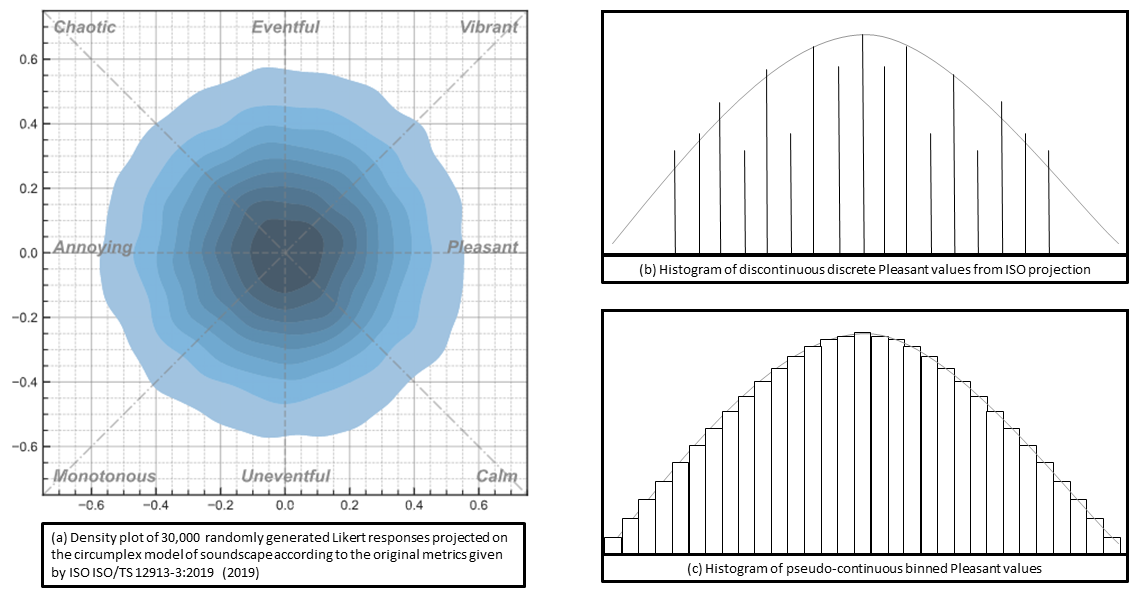
\includegraphics[width=\textwidth]{figures/Combined_sim_hist_mockup.png}
  \caption{Mockup placeholder simulation heatmap plot from Lionello 2020 and discrete vs binned transformation values. For new one, need to include distribution histograms along each axis.%
    \label{fig:isoheatmap}
  }
\end{figure}

Two important observations can be made about the shape of the resulting two-dimensional distribution. The first is that the shape of the available space is a circle. It should be noted that, despite what the term 'circumplex' may indicate, the perceptual dimensions are not necessarily intended to circumscribe a circle. The second is that, in each dimension, the responses are normally distributed, centered around zero. These points will be discussed in detail below.

\subsection{Circular space discussion}
%TODO: fill in circular discussion.
Visualisations of the circumplex model in soundscape literature tend to present it as circumscribing a circle (see Figure 1 in \citep{Axelsson2010principal} and Figure 3 in \citep{Torresin2020Indoor}), and this shape is further emphasised by the initial figure in \citet{Russell1980circumplex}'s original formulation of the concept. However, it should be emphatically noted that all of these presentations are in fact artefacts of the analysis methods which generated them, not some sort of revealed pattern in the component attributes which make up the circumplex. In \citet{Russell1980circumplex}, this first figure is generated by asking respondents to place each of the 27 attributes around a circle, according to their perceived spatial relationships - the circle shape was pre-imposed on the study. In both \citet{Axelsson2010principal} and \citet{Torresin2020Indoor}, the figures are generated via Principle Components Analysis (PCA) which, again, presents these results superimposed on a circle. It is perhaps a weakness of these two, otherwise strong and impactful, papers, that they did not recognise this consequence and challenge the circular arrangement.

If we turn back to Russell's original work on the circumplex model of affect, we can see some indications that a circle does not, in fact, describe the spatial relationship of the perceptual attributes. Fig. 4 of \citep{Russell1980circumplex}, which did not pre-impose the circular arrangement in its analysis, instead most closely resembles a square with rounded corners. Continuing from this conception, when Russell presents a graphical method of assessing the two dimensions of affect (pleasure and arousal) \citep{Russell1989Affect}, they use a square grid. This is all to say that, although the term 'circumplex' and the foundational analyses which lead to a soundscape circumplex may lead us to assume it must take the form of a circle, both the framework laid down by Russell and the common treatment of the spatial relationships of the attributes actually describe a square, instead.

This treatment of the 8 PAs makes several assumptions and inferences about the relationships between the dimensions. As stated in the standard \citep[p. 5]{ISO12913Part3}:

\begin{quote}
  According to the two-dimensional model, vibrant soundscapes are both pleasant and eventful, chaotic soundscapes are both eventful and unpleasant, monotonous soundscapes are both unpleasant and uneventful, and finally calm soundscapes are both uneventful and pleasant.
\end{quote}

From this, we would infer that a maximally vibrant soundscape is both maximally pleasant and maximally eventful. However, when the projection transformation is applied it imposes certain limitations on the relationships between the dimensions which do not conform with this assumption. As shown in \cref{fig:radar}, when a soundscape is maximally vibrant (i.e. a diagonal vector distance of 1), the maximum pleasantness value it can have is determined by the $\cos 45\degree$ term, giving a max pleasantness value of $\sim0.7071$. The implication of this is that no soundscape can be both maximally pleasant and maximally eventful at the same time, meaning that these dimensions are not in fact considered as orthogonal, and that a highly vibrant soundscape cannot be considered highly pleasant or highly eventful. Similarly, if a soundscape were to begin at a maximum Eventfulness, with neutral Pleasantness, in order for the soundscape to become more pleasant, it must by definition become less eventful. This is not conceptually correct or borne out in the treatments of previous literature. These same relationships and violations hold true for the other diagonal dimensions, chaotic, calm, and monotonous.

This implication violates both the assumptions made within the formulation of the circumplex model and the way that soundscape practitioners have understood and presented the interpretations of soundscapes within the circumplex space. In cases where the PA dimensions are referred to directly \citep{Steele2016Evaluation, Steele2019Soundtracking} and those which have made use of the Part 3 transformation to 2-dimensional coordinates \citep{Mancini2021Soundwalk, Lionello2021Introducing, Manzano2021importance}, \emph{Check Manzano2021importance} the conflation of maximal values on the diagonal axes with maximal values on the primary axes is made, as in the assumptions made by the standard. This is the first of the common understandings of the circumplex which are violated by the trigonometric transformation.

\subsection{Normal distribution discussion}
%TODO: fill in normal discussion

We can also see from the histograms included along the axes of \cref{fig:isoheatmap} that the projection creates a normal distribution in both dimensions. % TODO: edit this phrasing to match the final figure
It is important here to remember that the input to the projection formulas were uniform distributions for each of the 8 PAs, and it is the projection into the two primary dimensions which results in this normal distribution.
From the simulated distributions, we can derive a normal probability density distribution (PDF) for each of the dimensions.

\[   f_X(x) = \frac{x^{-(x-\mu)^2/(2\sigma^2)}}{\sigma \sqrt{2\pi}}\]
% ! TODO: Need to pull the actual standard deviation value.
with a mean $\mu = 0$ and standard deviation $\sigma = 0.3$.

\paragraph*{Realistic max values}
\draft{Review this}
% ! TODO: Andrew update this with the actual values from the calculations!
When looking at the distribution heatmap in \cref{fig:isoheatmap}, it is useful to picture the gradients as representing the available space in the circumplex model. The probability of reaching a given result decreases as we move farther away from the origin. This means, for example, that the probability of getting a pleasantness value between 0.2 and 0.3 is nearly 4 times the probability of getting a value between 0.5 and 0.6. This may not seem important, but the consequence is that, as a result of strictly the projection calculation, neutral values within the soundscape circumplex are much more likely and the space available to compare soundscapes within is truncated.

When we start to think about real-world urban soundscape data collection, where the discussion of the soundscape of a space is not limited to a single person's perception, we need to start thinking in statistical terms. Theoretically, the limits of the projected Pleasantness are (-1, +1), however according to the PDF calculated above less than 10\% of values fall outside the range (-0.5, +0.5).
% Note: Maybe this should be moved to Proposals or Discussion section?
It may be argued that as long as +1 can theoretically be reached, this should be what is considered the maximum value for that dimension. However, in any situation which involves using multiple individual soundscape assessments in order to characterize the overall soundscape of a location, this max will effectively never be reached. According to the large-scale, multi-location data set reported in our previous study, it appears that the effective maximum values for Pleasantness and Eventfulness for the combined assessment of multiple people for a space is in reality approximately (-0.6, +0.6) \citep{Lionello2021Introducing}.

As such, extreme values on each of the perceptual dimensions are less likely to occur than are coordinate values which place the soundscape in the neutral areas of the circumplex space. This means an extremely calm (or chaotic, or vibrant, or pleasant) coordinate is significantly less likely to occur than a neutral coordinate.


\subsection{Non-continuous projected values}
\draft{May want to remove this}
% Very brief presentation of this potential issue
An implicit assumption of the transformation is that the resulting coordinates are now continuous values, which allows linear regression and correlation methods to be used. Indeed, the transformation of the 8-dimensional ordinal Likert scale data to the two-dimensional coordinates creates a higher resolution of intervals, which would appear to be pseudo-continuous. Upon further investigation, the transformation actually results in XX discrete possible values. \cref{fig:isoheatmap}(b) shows a histogram of this raw output from the transformation, demonstrating that these discrete values, while following the general normal distribution discussed above, are not evenly filled - some adjacent values may be much more or less likely than their neighbours. This poses potential issues for further analysis which assumes either continuous or equally-spaced discrete values.
